\documentclass{article}
\usepackage[utf8]{inputenc}
\usepackage{amssymb}
\usepackage{tikz}
\usepackage{amsmath}
\usepackage{relsize}
\usepackage{mathtools}
\usepackage{textcomp}
\usepackage{eurosym}
\usepackage{amssymb}
\usepackage{systeme}
\usepackage{mathtools}
\usepackage[colorinlistoftodos]{todonotes}
\usepackage[
    backend=biber,
    style=apa,
  ]{biblatex}

\addbibresource{references.bib}
\title{Literature Review}
\author{Roman Oort}
\date{\today}

%%% PERSONAL SHORTCUTS
\DeclareMathOperator*{\plim}{plim}
\newcommand{\T}{\textbf{T}}
\newcommand{\Tij}{\textbf{T}_{ij}}
\newcommand{\Soc}{(\T(n))^{\infty}_{n=1}}
\newcommand{\beli}[3][2]{p_{#2}^{(#3)}}
\newcommand{\belvec}[2]{\textbf{p}^{(#2)}}

\begin{document}

\maketitle

\tableofcontents

\newpage

\section{Literature Review}
\todo{As it is still a draft I have not spent too much time on page layout, etc, as this is bound to change anyway}
\subsection{Social Learning}
Social learning is a field of study used in various different disciplines, ranging from economy to psychology, concerning the beliefs of agents in groups, and how these beliefs evolve and change over time. \cite{reed2010sociallearning}. Research in this field is dedicated to determining how individuals, and groups as a whole, change their beliefs and actions based on beliefs and actions of those around them. Many models have been proposed to formalize this process \cite{golub2017learning}, with the DeGroot model being one of the most prominent \cite{degroot1974concensus}.

\subsection{DeGroot Model}
\subsubsection{Agent Interaction}
A DeGroot model (\cite{degroot1974concensus}) consists of a set of $N=\{1, 2, ..., n\}$ of agents, interacting and exchanging information, and an $n \times n$ \emph{interaction} matrix $\T$ describing the nature of these interactions: whose opinions are heeded by whom, and how much so. Finally, the model also contains a belief vector $\textbf{p}$, which will be elaborated on in \ref{beliefs}. If the entry in the interaction matrix $\Tij > 0$ it indicates that agent $i$ listens to agent $j$, and the value of this entry determines how much weight agent $i$ places on agents $j$'s opinion: the higher this value, the more important $j$'s opinion is to $i$. It is important to note that $\T$ is a positive matrix, meaning it is not possible for an agent to place a negative weight on another agents opinion, they are only ever capable of ignoring other agents, or agreeing with them in some manner. 

Furthermore, the weight matrix $\T$ is a row-stochastic matrix, meaning that its rows sum to one:
\begin{align*}
    \sum_{j=1}^{n} \Tij = 1
\end{align*}

Finally, the matrix $\T$ is not necessarily symmetrical, making it entirely possible for an agent $i$ to hold the opinion of agent $j$ in high regard, while in return $j$ thinks very little of $i$'s opinion, or not even anything  at all.

\newpage

\subsubsection{Belief \& Learning}
\label{beliefs}

The belief of an agent $i \in N$ at a time $t \in \{0, 1, 2, ...\}$ is denoted as $p_{i}^{(t)}$, where this belief is taken as a real number on the interval $[0, 1]$. At the start of the process, at $t=0$, each agent $i$ is given a personal belief, through a private signal:
\begin{align*}
    \beli{i}{0} = \mu + e_i
\end{align*}
where $\mu$ is a real number, again on the interval $[0, 1]$, assumed to be the true state of the network, and $e_i$ is the random, zero mean, noise of agent $i$'s signal. \newline
The beliefs of all agents are aggregated into the belief vector $\textbf{p}^{(t)}$, where the $i$'th entry corresponds to the belief of agent $i$, at time $t$.

As time progresses the agents in the network update their own belief based on the beliefs of the agents around them, using the following updating rule:
\begin{equation}
    \label{updating:standard}
    \textbf{p}^{(t)} = \T\textbf{p}^{(t-1)}
\end{equation}
which means that the beliefs of all agents, at any time $t$, can simply be computed as the matrix multiplication of the interaction matrix and the belief vector at time $t-1$. How a single agent $i$'s opinion changes from $t-1$ to $t$ is then determined with the following calculation:
\begin{align*}
    \beli{i}{t} = \sum_{j=1}^{n}\Tij\beli{j}{t-1}
\end{align*}
which simply amounts to the weighted sum of the beliefs of all neighbours of agent $i$, where agent $i$'s neighbours are those agents $j$ to whom $i$ listens.

Furthermore, it is possible to compute the belief vector $\textbf{p}^{(t)}$, without computing the belief vector at every preceding $t^\prime < t$, the formula for which can be derived from equation \ref{updating:standard}, as follows:
\begin{align*}
    \textbf{p}^{(t)} &= \T\textbf{p}^{(t-1)} \\
    &= \T\T\textbf{p}^{(t-2)}\\
    &= \T^2\textbf{p}^{(t-2)}\\
    &= \T^3\textbf{p}^{(t-3)} \\
    & \ \ \ \ \ \  \vdots \\
    &= \T^{t}\textbf{p}^{(0)}
\end{align*}
In other words, the belief vector at time $t$ can be computed by multiplying the interaction matrix $\T$ with itself $t$ times, and multiplying the resulting matrix with the initial belief vector.
\newpage

\subsubsection{Convergence}
\label{convergence}
As we are interested in the spread of information through the network, and whether or not the agents in a network will learn the supposed true state of the world, an important notion is the concept of \emph{convergence}. The interaction matrix $\T$ is said to be convergent if:
\begin{equation*}
    \lim_{t\to\infty} \T^t\textbf{p}
\end{equation*}
exists for all $\textbf{p} \in [0, 1]^n$. That is to say, as time progresses sufficiently, the beliefs of the agents, independent of their starting signal, approach a constant value and no longer change.

Another important property is \emph{aperiodicity}, which concerns cycles: paths through the network that start and end at the same agent. A network is said to be aperiodic if the largest common divisor of the length of all cycles in the network is no more than 1. This condition is automatically satisfied as long as there is at least one agent present in the network who has a link to themselves, as this creates a cycle of length one, ensuring there can be no common divisor larger than one.

A final notion important in the convergence of social networks is \emph{connectedness}. When applied to undirected networks, wherein a link between two agents works both ways, a network is said to be connected when there exists some path between any two agents $i$ and $j$. However, when applied to \emph{directed} networks this notion changes slightly, and can be divided in two distinct notions, more specifically, a connected directed network can be either \emph{weakly} or \emph{strongly} connected. A directed network is said to weakly connected if there exists some undirected path between any two agents in the network. However, if there also exists a \emph{directed} path between any two agents, a directed network is said to be strongly connected.

Now, assuming that \T, is the interaction matrix of a strongly connected network, the following three statements are equivalent:
\begin{itemize}
    \item[-] $\T$ is convergent
    \item[-] $\T$ is aperiodic
    \item[-] There is some unique left eigenvector, \textbf{s}, of \T, corresponding to the eigenvalue $\lambda=1$, such that, for every \textbf{p}$\in [0,1]^n$, and every agent $i$,
    \begin{align*}
        (\lim_{t\to\infty}\T^t\textbf{p})_i = \textbf{sp}
    \end{align*}
\end{itemize}

 This last eigenvector property not only provides a definition of convergence, but also the actual convergent belief of the network, which is nothing more than a multiplication of the left eigenvector, also called the influence vector, \textbf{s} and the belief vector \textbf{p}. Furthermore, as \textbf{s} is a $1 \times n$ row-vector, and \textbf{p} an $n \times 1$ column-vector, their multiplication results in a single number, highlighting that there is one single, universal, convergent belief.

\newpage

\subsubsection{Wisdom of Crowds}

Having established the convergence property for social networks it becomes possible to look towards the notion of wisdom, central in \cite{golub2010naive}. They defined wisdom to mean that a given network not only converges, but converges to the assumed true state of the model, $\mu$, specifically in the context of large societies. This means they are looking at networks where the number of agents in the network $n\to\infty$.

To encapsulate the idea of large societies, providing insight in the behaviour of these models as the participating number of agents becomes sufficiently large, limiting statements with regard to the number of agents are used. To this end a society is defined as a sequence of networks, indexed by the number of agents in the network, $n$: $\Soc$. This means that the entry $\textbf{T}(n)$ is the interaction matrix of the network in the sequence with $n$ agents, where $\textbf{T}(n)_{ij}$ is used to denote the entry $(i,j)$ in this specific sequence. A similar method of indexing is applied to all previously discussed properties of these networks, i.e.: belief vectors, influence vectors.

The beliefs of the agents are generated using the same mechanism described in section \ref{beliefs}, i.e.: independently distributed zero mean error terms added to the assumed truth, where $\beli{i}{t}(n)$ is used to indicate the belief of agent $i$ at time $t$ in a network with $n$ agents. Under the assumption that every network in our given sequence converges, we write the convergent belief of an agent $i$, that is to say the belief as $t \to\infty$, as $\beli{i}{\infty}(n)$, as described in \ref{convergence}.

Using these notations a sequence $\Soc$ is deemed to be wise if:
\begin{equation}
    \label{wisdom:equation}
    \plim_{n\to\infty}\max_{i \leq n}|\beli{i}{\infty}(n) - \mu| = 0
\end{equation}
That is to say, a sequence of network is wise if, as $n$ becomes sufficiently large, the convergent belief of \emph{every} agent in the network is equal to the truth, which, using the fact that the convergent belief can be computed using the influence vector \textbf{s} can be rewritten as:
\begin{equation}
    \label{wisdom:influence}
    \plim_{n\to\infty} \textbf{s}(n)\textbf{p}^{(0)}(n) = \mu
\end{equation}
which holds if and only if $s_{1}(n) \to 0$, where $s_1(n)$ is the first entry in the \emph{ordered} influence vector \textbf{s}. In other words, a sequence of networks if wise if and only if the influence of the most influential agent tends to zero, as $n$ becomes sufficiently large.

\newpage

\subsection{Obstructions to Wisdom}
\todo{I am thinking this is probably the section were the most can be cut, as the focus in the implementation is on the non-coop agents.}
While the wisdom of crowds effect is a powerful notion, it is not infallible. Most notably, it is also a fragile concept, with many factors capable of disrupting the network's ability to obtain wisdom. Some of these factors are consequences of the structure of the networks, while other are caused by agents who purposefully refuse to participate in the exchange of information.

\subsubsection{Prominent Families}

One general obstacle to the convergence to wisdom is similar to requirement of vanishing influence of individual agents. Namely, the existence of groups, in the network that are disproportionally influential over other groups.
This means that the existence of a group in the network with a disproportional sway over the rest of the network can steer the entirety of the network away from the truth, just as a single over-influential agent can.

To reason about the influence of groups first an actual definition of the influence of a group is necessary, as all previously mentioned notions of influence were applied only on the scale of individual agents. To this end, let $B$ and $C$ be two groups in the network s.t. $B \subset N$, $C \subset N$ , where $N$ is the set of all agents in the network, then the weight that group $B$ places on $C$ is defined as follows:
\begin{equation}
    \textbf{T}_{B, C} = \sum_{i\in B}\sum_{j \in C} \Tij
\end{equation}
Simply put: the total weight of a group $C$ on another group $B$ is simply the sum of all incoming weights to agents in $B$ from agents in $C$.

Another measure used to describe the influence of groups is the prominence of a group, which is a measure of a group's influence respective to the entire network, rather than one single group.
A group $B$ is said to be prominent, at a given $t$, if every agent $i \notin B$ in the network listens to some agent $j\in B$, at that $t$.
A group $B$ is therefore said to be prominent in $t$ steps, relative to a network, if,for every $i \notin B$, $(\textbf{T}^{t})_{i,B} > 0$. An important property based on this notion is the $t$-step prominence of B relative to \textbf{T}: 
\begin{equation}
    \pi_B(\textbf{T}; t) = \min_{i\notin B} (\textbf{T}^{t})_{i,B}
\end{equation}
This is the smallest weight that is placed on some agent in the group $B$, by any agent $i\notin B$. Therefore this value will only be larger than zero for any values $t \geq t^{\prime}$, where $t^{\prime}$ is the smallest t for which
the group $B$ is prominent relative to the network.
\newline

However, these definitions of groups are defined only on single networks, while, in the context of wisdom, the interest lies in sequences of networks. The notion of groups can be slightly expanded to be useful in the context of societies. For this purpose a family is defined as a sequence of groups $(B_n)$, where each $B_n \subset \{1, ..., n\}$, such that each group in the sequence is a subset of the agents present in the network of that size $n$.

Having extended the notion of groups to the context of societies the prominence measure can be expanded in a similar manner. Namely, a family $(B_n)$ is said to to uniformly prominent relative to $\Soc$ if there exists a constant, $\alpha$, and there is a $t$ such that $B_n$ is prominent in $t$ steps relative to $\T(n)$, and $\pi_B(\textbf{T}; t) \geq \alpha$, for every $n$. In other words, for a family $B_n$ to be uniformly prominent it has to have a minimum influence greater than $\alpha$ over each individual agent $i$ outside of $B_n$, at every size $n$ of the society.

\noindent Finally, a family $(B_n)$ is called finite if there exists some $q$ such that:
\begin{equation*}
    \sup_n |B_n| \leq q
\end{equation*}
Or, in other words, a finite family is a family that has a finite upper bound on its members.

Now, it is the case that the disproportional influence of groups can cause a network no longer to be wise, namely, the presence of finite, uniformly prominent family relative to the society $\Soc$, prevents this society from becoming wise.

\subsubsection{Non-cooperative Agents}
\label{non-coop}
Another factor capable of preventing wisdom in a network is the presence of a non-cooperative agent in the network (\cite{amir2021robust}). That is to say, an agent in the network not adhering to the regular updating mechanics, deliberately spreading misinformation to its neighbours. The presence of even one of these non-cooperative agents in  the network is enough to prevent wisdom in the network. \footnote{Assuming the private belief of this agent is not equal to the assumed truth.} Even though a network may satisfy all the necessary conditions required for wisdom this one agent not playing by the rules will steer the network away from, what otherwise would have been, the convergent belief. In fact, not only will this agent prevent the other agents from converging to the truth, they also make all other agents converge to the belief of this non-cooperative agent (\cite{amir2021robust}).

\subsubsection{Structural Obstructions}

Finally there are some obstructions that prevent the occurrence of wisdom in a given society that are more dependent on the actual structure of the network rather than the weights on the links or adherence to the updating rules (\cite{jackson2010social}). Determining these conditions requires some more notions about the structures of the network, the first being the notion of balance. For a network to be considered balanced there must be a sequence $j(n) \to \infty$, such that if $|B_n| \leq j(n)$ then:
\begin{equation}
    \sup_n \frac{\T_{B^c_n, B_n}(n)}{\T_{B_n, B^c_n}(n)} < \infty
\end{equation}
That is to say, for a network to be balanced, as the network, and this group $B$, grow, the amount of attention paid to said group by outside agents cannot be infinitely many times larger than the weight placed on the outside agents by the agents that \emph{are} part of this group.
This notion captures the idea that a group cannot be too self-centered, paying very little attention to what others outside of that group are saying. However this only needs to hold for groups smaller than indicated by the sequence $j(n) \to\infty$, which can increase arbitrarily slow, rendering it relatively harmless.
This property is a natural extension of the idea that one single agent should not be getting infinitely more weight than they are placing on other agents, but applied to groups rather than individual agents. \newline

However, balance alone is not enough to ensure a wise network. Another important, structural, measure is the minimal out-dispersion. This condition states that there exists some $q\in \mathbb{N}$ and $r > 0$, such that if $B_n$ is a finite group, $|B_n|\geq q$ and $\frac{|C_n|}{n}\to 1$, then $\textbf{T}_{B_n, C_n} > r$, as $n$ becomes sufficiently large. Simply put, this condition requires that any finite group of a given size must place a minimal amount of weight on a group consisting of nearly the entire network. This prevents smaller groups to remain in their own isolated clusters, focusing almost all their attention inwards, ignoring the vast majority of the network.

With these two condition in place it is possible to formulate a sufficient condition for wisdom, namely, that if a society $\Soc$ satisfies \emph{both} balance and minimal out-dispersion, it is wise.

\subsection{Variations}

As mentioned in \ref{non-coop} the presence of non-cooperative agents in the network is greatly disruptive for the ability of a network to attain wisdom. So much so, even, that only one non-cooperative agent is sufficient to prevent any network, regardless of size, from attaining wisdom. Furthermore, not only does this agent prevent wisdom, they also ensure that the final convergent belief of the network will be equal to their own belief, with regard for neither the initial beliefs of the cooperative agents, nor the assumed truth of the network. As the presence of even one such agent disrupts the wisdom of the entire network research is done on how to make the standard, \emph{naive}, DeGroot model more resilient to the presence of such non-cooperative agents. Several variations of the DeGroot model, and how they distinguish themselves from the standard model, will be discussed.

\subsubsection{$\varepsilon$-DeGroot}

One such variation, specifically designed by \cite{amir2021robust} to combat the presence of such non-cooperative agents in the network, is called $\varepsilon$-DeGroot. This variation makes a small adjustment to the standard updating rule of the DeGroot model, in an attempt to achieve wisdom, despite any non-cooperative agents present in the network.

In the standard DeGroot model an agent's belief at time $t$ is simply the weighted sum of their neighbours' opinions, according to \ref{beliefs}, with no limit on how much an agent can change their opinion in a single time-step. In contrast, in the $\varepsilon$-DeGroot model, the parameter $\varepsilon$ is used as a threshold in the updating step to prevent agents from changing their belief drastically in a single time-step.
Instead of simply updating their current opinion, $x$, to the weighted sum of their neighbours' opinions, $y$, they check whether the difference between the two falls under the threshold before updating their opinion, changing the updating rule from equation \ref{updating:standard} to:

\begin{equation}
    \label{edegroot:updating}
  \beli{i}{t} =\Bigg\{
  \begin{matrix*}[l]
  y \text{ if } |\beli{i}{t-1} - y| \leq \varepsilon\\
  y^{\prime}\in\{y-\varepsilon, y+\varepsilon\}\text{ s.t. }|\beli{i}{t-1} - y^{\prime}|\text{ is minimized, otherwise}
  \end{matrix*}
\end{equation}
where $y = (\textbf{T}\textbf{p}^{t-1})_i$. This means that at each $t$ each agent $i$ does not indiscriminately change their opinion to the combined opinion of their neighbours, as with regular DeGroot mechanics. Rather, they check whether the difference between this combined belief and their own, previous, belief, falls under a certain threshold, given by $\varepsilon$. If so, they take this combined opinion, otherwise they change their opinion to the closest of $\{y-\varepsilon, y+\varepsilon\}$. So, the larger $\varepsilon$ is chosen, the more an agent can change their opinion in a single updating step, and the smaller this $\varepsilon$ is chosen, the more this rule approaches the standard DeGroot updating process. After all, if $\varepsilon = 0$ the updating rule becomes\todo{Not sure if it is necessary to show this explicitly}:
\begin{equation*}
  \beli{i}{t} =\Bigg\{
  \begin{matrix*}[l]
  y \text{ if } |\beli{i}{t-1} - y| \leq 0\\
  y^{\prime}\in\{y\}\text{ s.t. }|\beli{i}{t-1} - y^{\prime}|\text{ is minimized, otherwise}
  \end{matrix*}
\end{equation*}

Using an updated metric for the learning process, called $(\delta, \rho)$-learning, which is achieved by that agent if their opinions falls with in $\delta$ of the assumed truth, $\mu$, with probability $1 - \rho$. On an infinite graph this condition is satisfied when all but a finite group of agents satisfy this condition.\todo{Not sure whether to mention this, as this metric is really only useful in the context of infinite networks} \newline


\todo{Alternative method should probably be discussed in the method, as it does not directly stem from the literature}One thing to note is that the $\varepsilon$-DeGroot dynamics as described above do not impose a hard, uniform, limit on how much an agent's opinion can change. But rather, this maximum change is determined by the new belief of each agent, and therefore varies from agent to agent. Therefore an alternate approach to the $\varepsilon$-DeGroot dynamics would be to base the new opinion, should the difference between the currently held opinion and the newly computed one exceed the threshold, on the currently held opinion, rather than the newly computed one, changing the updating rule to:
\begin{equation*}
    \label{edegroot:alt}
    \beli{i}{t} =\Bigg\{
    \begin{matrix*}[l]
        y \text{ if } |\beli{i}{t-1} - y| \leq \varepsilon\\
        x^{\prime}\in\{\beli{i}{t-1}-\varepsilon, \beli{i}{t-1}+\varepsilon\}\text{ s.t. }|y - x^{\prime}|\text{ is minimized, otherwise}
    \end{matrix*}
\end{equation*}
In other words, should the difference between the new opinion and the previous opinion exceed the threshold, $\varepsilon$ is simply added to, or subtracted from, the current opinion, whichever is closest to the belief as computed through the standard updating rule. This imposes a hard limit on how much an agents opinion can change in a single update, namely $\varepsilon$. This hard limit is universal for all agents in the network, instead of varying across different agents as is the case in the regular $\varepsilon$-DeGroot rule.

\subsubsection{Private Belief}

Another variation introduced by \cite{friedkin1990private}, permits each agent to hold on to persistent private belief. When updating each agent then not only considers the weighted sum of the beliefs of their neighbouring agents, but also take into account this private belief. Furthermore, this private belief does not change over time, but remains constant, making it distinct from an agents' link to themselves, should this self-link be present. This variation on the model changes the updating rule to the following:

\begin{equation}
    \beli{i}{t} = (1-\alpha_i)(\textbf{T}\textbf{p}^{(t-1)})_i + \alpha_i b_i
\end{equation}
where $b_i$ is the private belief of an agent $i$, of course on the interval $[0, 1]$, and $\alpha_i$ is the weight that said agent places on their private belief, also on the interval $[0, 1]$. In essence the updating rule becomes a weighted sum of the new belief, as computed through the standard updating rule, and an agent's private belief.

\subsubsection{Stochastic DeGroot}

One final variation on the standard DeGroot model that will be discussed is the \emph{stochastic} DeGroot model, introduced by \cite{chatterjee1977stochastic}. Rather than keeping the interaction matrix $\textbf{T}$ constant as $t \to \infty$, the stochastic DeGroot model allows this matrix $\textbf{T}$ to change over time. This alleviates one of the main shortcomings of the standard DeGroot model, which supposes that each agent will never change the weight they place on the opinions of their neighbours. Instead a stochastic DeGroot model allows the weights to evolve over time. This changes the updating rule to the following:
\begin{equation*}
    \beli{i}{t} =(\textbf{T}(t)\textbf{p}^{(t-1)})_i
\end{equation*}
The idea of the updating rules remains the same, the only difference being that the weight matrix $\textbf{T}$ now also varies over time, rather than being constant.

\newpage

\section{Network Generation}

\subsection{Random Generation}
\label{generation:random}
In order to allow for proper analysis of the DeGroot mechanics a method to generate \emph{random} networks was created, to ensure generality of the obtained results. Given a number of agents this method is capable of generating both directed and undirected networks, and accepts several other parameters to shape the generation as desired.

\subsubsection{Default Case}
In the default, most basic, case this function simply takes the desired number of agents, $n$ as input. Other, optional, parameters can be provided to customize the desired network and will be discussed in detail at the relevant time.
To start, an empty $n\times n$ array \cite{2020NumPy-Array}, i.e. containing solely zeroes, is created, which serves as a blank slate for the interaction matrix $\T$ of the network.
Subsequently the function will iteratively add the links for every agent in the network, in order to ensure the generated network is fully connected at every size. \newline
In this iteration there is one special case, namely, the very first agent. To ensure aperiodicity, as discussed in [REF], and therefore convergence, the very first agent is guaranteed to receive a self-link. As this creates a cycle of length one, aperiodicity is guaranteed. \newline

Every subsequent agent, when generating a directed network, will be guaranteed to both receive and send one link. When generating an undirected network each agent is guaranteed to have one link, which is both incoming and outgoing. This guarantees that the network of size $n$ will be fully connected. However, as the interest lies in sequences of networks, all of which need to be convergent, this condition needs to be met by every network in the sequence of size $n^{\prime} < n$, not only by the network of size $n$. Therefore, these guaranteed links will be sent to, and by, an earlier agent in the network, that is to say that the guaranteed links of an agent $k$ can only be sent to and received by any agent $m < k$. This guarantees the strong connectedness of the network, at every size, which can be proven inductively, see section \ref{proof:conn}. This also holds for an undirected network, where the only difference is that the agents receiving and sending a link are one and the same. The specific agents on the other end of these guaranteed links are sampled randomly from a uniform distribution over the interval of agents already present in the network. \newline

Therefore, as this method of generation not only guarantees connectedness in the total network, but also at every smaller size of the network, this returned network can also be considered a sequence of networks. To access a network of a specific size in this sequence, one would only need to take the rows and columns up to that size to obtain the specific network. This ensures that the network and its links stay constant between sizes, allowing for proper comparison of different networks in the sequence. Finally, this function is also capable of growing an existing network: when a matrix and a positive integer $m$ are provided, the function will grow this existing matrix by adding $m$ rows and columns, one for each agent, whose links are determined in the same way as described earlier.\newline

This method of generating these network was chosen over more standard methods of model generation for several reasons. For starters, implementing the network generation from scratch provides more low-level control over the network generation process, allowing more options for customization. A clear effect is the strong connectedness mentioned earlier. Using another method for generating the network, while possibly faster when initially generating the network, would require another pass over all agents to ensure the network is fully connected, and remains so at every size. 

Another, more subtle, effect of the chosen method is a slight bias towards the earlier agents in the network, an effect which can be seen in figure (\ref{degree:agent}) below, which shows the average degree for each consecutive 100 agents. As shown earlier the agents are added to the network the higher their degree tends to be. This mirrors how those individuals who are part of a group for a long time tend to have more connection than those new to the group.

\begin{center}
    \begin{figure}[!htbp]
        \centering
        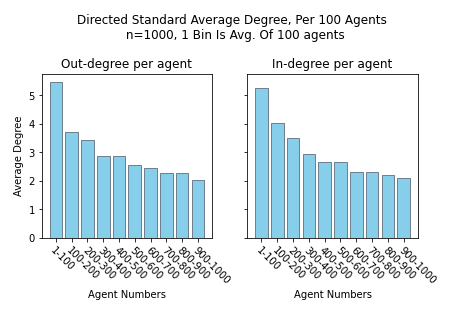
\includegraphics[width=.8\textwidth]{ThesisKI/Images/DirectedStandardPerAgent.png}
        \caption{Average Degree per 100 agents}
        \label{degree:agent}
    \end{figure}
\end{center}
\newpage
\subsubsection{Customization}

As mentioned the chosen implementation has the option to adjust the generation process as desired. These adjustment are applied complementary to the default generation, to ensure the base guarantees of this method. \newline

First of all, this method allows for the generation of both directed and undirected networks. The method for generating undirected networks is very similar to the generation of directed networks. In fact, the process is entirely the same, save for one detail. In contrast to the generation of a directed network, where the agents to receive and send a link are chosen independently, and therefore tend to be distinct agents, the generation of an undirected network simply chooses one random agent to both receive and send a link. After all, the only difference between the interaction matrix $\T$ of a directed and undirected network is that the matrix of an undirected is symmetrical, whereas the matrix of an undirected network is asymmetrical. \newline
Furthermore, when a directed network is created it can be made into an undirected network. This is done by simply taking the element wise maximum between the original matrix and its transpose, effectively mirroring all links in the matrix along the diagonal. \newline

Secondly, there is also the option to increase the degree of the agents to more than the base minimum. Using the default generation results in nearly half of all agents having only two links, the bare minimum \footnote{In a network where every agent is guaranteed a self-link}, with a quickly dissipating tail on this distribution as demonstrated in figure (\ref{deg:std}). However, when using this option to increase the degree of the network, this distribution is spread out more evenly and is flattened, leading to a more even distribution of degrees, as seen in figure (\ref{deg:inc})
\begin{figure}[!htbp]
  \centering
  \subfloat[Standard Degree]{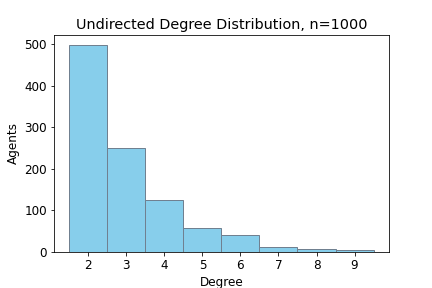
\includegraphics[width=0.5\textwidth]{ThesisKI/Images/DegreeUndirectedStd.png}\label{deg:std}}
  \hfill
  \subfloat[Increased Degree]{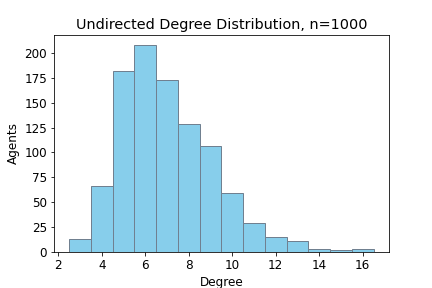
\includegraphics[width=0.5\textwidth]{ThesisKI/Images/DegreeUndirectedInc.png}\label{deg:inc}}
  \caption{Degree Distributions Undirected Network}
\end{figure}

\newpage

The procedure for increasing the degree of a network occurs during the generation procedure. During the iteration, each agent samples a random number to increase their degree by, sampled from a given distribution, by default $\mathcal{N}(2,1)$, which was also used to generate figure (\ref{deg:inc}). This number is then rounded to the nearest integer, and, when this integer is positive, the agent will receive this amount of additional links. Once again the agents on the other end of the link are sampled randomly from a uniform distribution, this time over \emph{all} agents, not only over those already present in the network, and the corresponding element in the matrix is then set to one. When this method is used for an undirected network only one number is drawn to increase the degree, however, for a directed network two number are sampled, for both the in-degree and the out-degree.
The probability distribution, and its respective parameters, from which the degree increase is sampled can be changed to influence the distribution of degree as much as desired.
\newline

A final option for the customization of the network generation is the probability of a self-link, which can be set at the moment of generation. This sets the probability for each agent to form a link with itself, save for the first agent, which always receives a self-link in order to ensure the aperiodicity of the network.
\begin{center}\todo{increase font-size}
    \begin{figure}[!htbp]
        \centering
        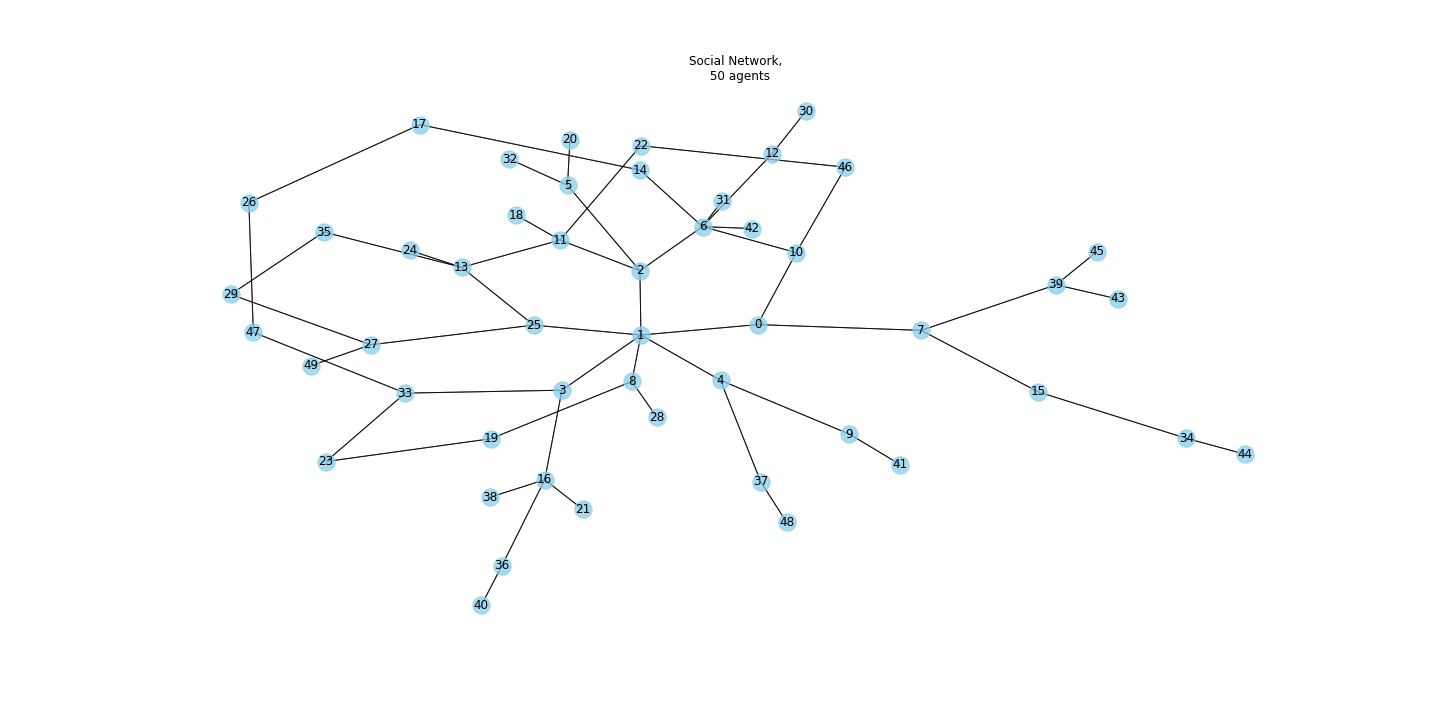
\includegraphics[width=1.1\textwidth]{ThesisKI/Images/NoneGraphRandom.png}
        \caption{Example of Randomly Generated Undirected Network}
        \label{network:random}
    \end{figure}
\end{center}

\newpage

\subsubsection{Sparse Matrices}

One caveat of the chosen implementation is the memory consumption. As the interaction matrix is two-dimensional its size increases in a polynomial manner. As the wisdom of crowds effects occurs as the network size approaches infinity this poses a problem, with large networks consuming a large amount of memory. In order to circumvent this problem the implementation of the network generation stores the interaction matrix in a sparse format \cite{2020SciPy-NMeth}. As can be seen in figure (\ref{generation:memory}) this decreases the memory consumption to negligible levels, for networks of up to $10,000$ agents, whereas when using a standard, dense, matrix the memory consumption increases rapidly. \newline
However, generating a network as a sparse matrix is a somewhat slower process than generating the same network as a dense matrix, though both generation processes still run in linear time as can be seen in figures (\ref{generation:time_inc} \& \ref{generation:time_std}),  which show the network generation times for a network with increased degree, and standard degree respectively. Therefore, as the generation of the network needs only be run once, the decrease in memory usage was considered to outweigh the slightly increased run-time, and the sparse generation was chosen as default.
\todo{increase font-size}
\begin{figure}[!htbp]
    \centering
    \subfloat[]{\label{generation:memory}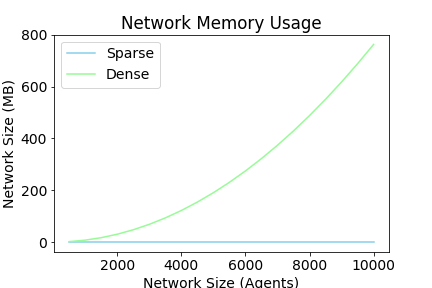
\includegraphics[scale=.45]{ThesisKI/Images/Memory.png}}
    
    \begin{minipage}{.5\linewidth}
    \centering
    \subfloat[]{\label{generation:time_inc}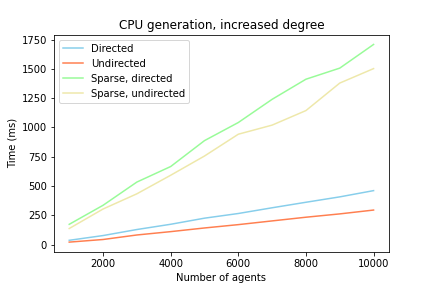
\includegraphics[scale=.4]{ThesisKI/Images/CPU_inc.png}}
    \end{minipage}%
    \begin{minipage}{.5\linewidth}
    \centering
    \subfloat[]{\label{generation:time_std}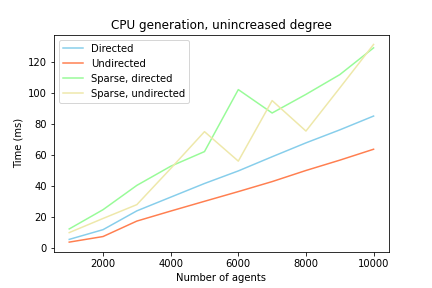
\includegraphics[scale=.4]{ThesisKI/Images/CPU.png}}
    \end{minipage}\par\medskip
    \caption{Network generation, \\ memory and time consumption}
\end{figure}


\section{Belief Initialization}

The generation of the beliefs follows the procedure as discussed in section [REF]. That is to say, the initial opinion of an agent $i$, $\beli{i}{0}$, is generated by adding a random, independently sampled, zero-mean, error term, $e_i$, to the assumed truth of the network. This is implemented by generating an array of length $n$, where each entry is sampled from a zero mean probability distribution, $\mathcal{N}(0, 0.75)$ by default. The assumed truth, $\mu$, is drawn randomly from a uniform distribution on the interval $[0, 1]$, and is added to each entry in this array of error terms. \newline
However, as mentioned in section [REF] all beliefs are to lie on the interval $[0, 1]$, which is not guaranteed with this method. After all, as $\mu$ is chosen randomly it can lie arbitrarily close to the edges of the interval, allowing for the a very small error term to push the belief outside of the interval. What's more, the probability distribution is continuous, meaning it is even possible for an error term to be larger than $1$.  Therefore, in order to force each belief onto this interval the initial belief vector is value normalized, according to following rule:
\begin{equation*}
    \beli{i, \text{norm}}{0} = \frac{\beli{i}{0} - \min(\textbf{p}^{(0)})}{\max(\textbf{p}^{(0)}) - \min(\textbf{p}^{(0)})},
\end{equation*}
which ensure that the smallest belief in the belief vector is normalized to $0$, the highest belief normalized to $1$, and every other belief will fall somewhere in between. However, as this shift the mean of the belief vector away from $\mu$, $\mu$ itself must undergo the same normalization in order to ensure each belief is still properly generated from this value.
\newline

\section{Weight Initialization}

The previous method does instantiate the network, by creating the links between all agents. However, it does not yet place a weight on all of these links, to describe how much weight agents place on the beliefs of others. For this purpose different options to initialize the weights have been determined. These are all applied only on the non-zero entries in the interaction matrix, therefore they do not create any new links, nor do they remove those already existing links, potentially disrupting the connectedness of the network.

\subsection{Uniform}

The first, default, weight initialization is uniform weighting. This simply means that every agent places the exact same weight on the opinions of every other they are connected to. The implementation amounts to simply let the interaction matrix $\T$ remain as is, with a $1$ indicating a link and a $0$ indicating no link.

\subsection{Overlap}

The second initialization is based on the idea that an agent prefers to receive information from as many different sources as possible. The weight placed on an agent is therefore proportional to the amount of new information they are able to provide, based on the overlap in neighbours between two agents, where agents' neighbours are those other agents with whom they have a link. The weight initialization is based on the following rule:
\begin{equation*}
    \T_{ij}(n) = 1 - \alpha \cdot \frac{|N_i(n) \cap N_j(n)|}{|N_i(n)|},
\end{equation*}
which essentially subtracts the fraction of overlap between the set of neighbours of agents $i$ and $j$ from the weight that $i$ places on $j$. This fraction is then multiplied with a discount factor $\alpha \in [0, 1)$ to ensure that a link between agents is not deleted in the event that their neighbouring sets perfectly overlap. 

\subsection{Belief}

Another method of setting the weights between agents is based on the idea that agents are more willing to pay attention to those around them with the same mindset. The weight that one agent places on another is based on their difference in opinion: the more similar their opinions the more weight they attribute to the other's opinion, and vice versa. First, in order to set the weights this way, the initial belief vector is concatenated with itself $n$ times, to form an $n \times n$ matrix where each column is the belief vector at $t=0$, as follows:
\begin{equation}
    B(n) = [\textbf{p}^{(0)}(n)]^{n},
\end{equation}

In order to get the difference in belief between any two agents, the transpose of the matrix formed by concatenating the belief vectors can simply be subtracted from the matrix itself. Then, for every non-zero element in $\T$, the weight is set as the absolute difference in opinion subtracted from 1, as follows:
\begin{equation*}
    \T_{ij}(n) = 1 - \alpha \cdot |B_{ij}(n) - (B^{T})_{ij}(n)|,
\end{equation*}

Again, just as in the overlap initialization, $\alpha$ is a discount factor on the interval $[0, 1)$ to prevent deletion of links, should two connected agents hold perfectly opposed beliefs.

\subsection{Random}

Another method of initializing the weights of the network is to simply generate the the weights randomly. This method generates an $n \times n$ matrix filled with numbers sampled from a given distribution, and corresponding parameters, a uniform distribution on $[0, 1]$ by default. In order to ensure the weights are applied only to existing links the randomly generated matrix and the interaction matrix $\T$ are multiplied element-wise, as each element of the $\T$ matrix at this point is either $1$ or $0$.

\subsection{Self-links}

One final hiccup in the weight initialization are the self-links. When using either uniform or random weights everything works as intended. However, when setting the weight based on either overlap of belief unintended behaviour occurs. Namely, when setting the weights based on overlap, a self-link will always be assigned the lowest possible weight. After all, two identical sets, in this case the overlap between the sets of neighbours of agents $i$ and $i$, will perfectly overlap.
Conversely, when setting the weights based on beliefs, a self-link will always receive the highest possible weight. After all, the difference in opinion between an agent and themselves will always be $0$. \newline
In order to circumvent this, when initializing the weights using one of the aforementioned methods, the self-links will be assigned a random weight, sampled from a normal distribution whose mean and standard deviation are taken to be the mean and standard deviation of all other weights in the network. This ensures that the self-links are generated to be more in line with all other weights in the network.

\subsection{Normalization}

Finally, in order to achieve convergence, it is necessary that $\T$ is row-stochastic, meaning its elements sum to one, row-wise. In order to ensure this condition, after the weights have been initialized, the matrix is normalized row-wise as follows:
\begin{equation*}
    \T_{ij, norm}(n) = \frac{\T_{ij}(n)}{\sum_{j}\T_{ij}(n)},
\end{equation*}

In other words, each entry is simply divided by the sum of all weights in the corresponding rows. While this does not preserve the exact values given to the weights by the initialization function, it does preserve their values in relation to the other weights in the row, which is the most important.

\newpage

\section{Non-cooperative Agents}

Now, having the ability to generate a cooperative network of a given size, what remains is the ability to add non-cooperative agents without disrupting the benefits obtained by the chosen method of network generation.
Furthermore the implementation has to have the ability to switch a network between cooperative and non-cooperative at will, to allow for proper comparison between those networks.
Therefore the generation of the non-cooperative agents occurs after the cooperative part of the network has already been generated. Iterating over the given number of non-cooperative agents, each of them receives a random selection of agents with whom they will have a link, the number of which will be equal to the average degree of the network, at its full size.
In addition to the randomly selected agents each non-cooperative agent is guaranteed to receive a link to one of the first five agents in the network. This is done to make sure that the non-cooperative agents will still have links to others, even when the observed network is relatively small.

The links of these non-cooperative agents are then stored to allow them to be added to a network of any size. In order to add them to any network in the sequence, regardless of size, first empty rows are concatenated to the interaction matrix. After all, what distinguishes non-cooperative agents from their cooperative counterparts is their lack of incoming links, expressed by empty rows in the interaction matrix. After the empty rows are added, the respective columns are added, representing those agents who listen to non-cooperative agents. The regular interaction matrix of size $n \times n$ is therefore extended to a matrix of size $n+m \times n+m$, where $m$ is the number of non-cooperative agents.
An example of a resulting non-cooperative network can be seen in figure (\ref{network:noncoop}), below, where the non-cooperative agents are labeled in red.

\begin{center}\todo{increase font-size}
    \begin{figure}[!htbp]
        \centering
        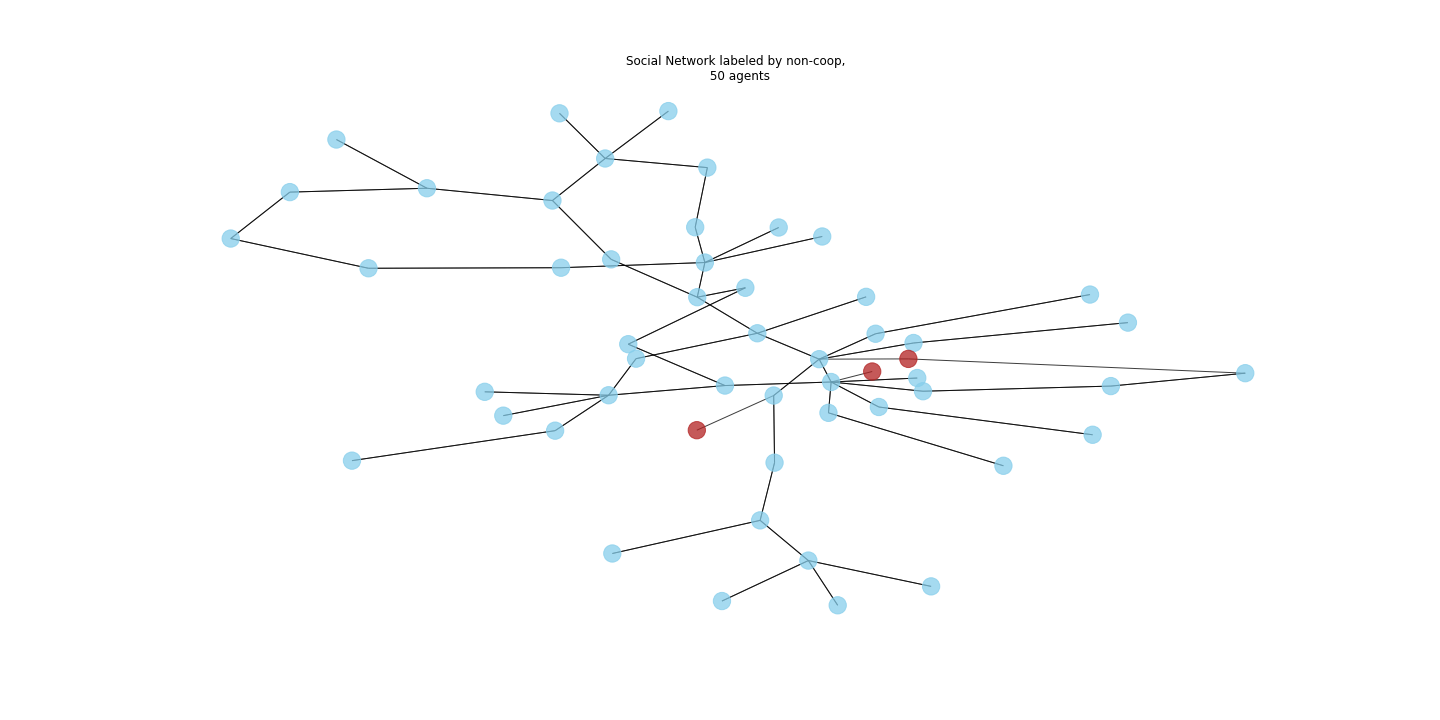
\includegraphics[width=1\textwidth]{ThesisKI/Images/NonCoopGraph.png}
        \caption{Non-cooperative network, $n=50, m=3$}
        \label{network:noncoop}
    \end{figure}
\end{center}


\newpage


\section{Updating Rules \& Convergence}

In order to compare the different variations on the DeGroot mechanics these variations all needed their respective updating rules to be implemented.

\subsection{DeGroot}

As shown in section [REF]\todo{ref naar updating rule section} $\textbf{p}^{(t)}$ can be computed two different ways. The first is the iterative method described in equation [REF] \todo{ref naar iterative updating method}, simply multiplying the belief vector at the previous time-step, $\textbf{p}^{(t-1)}$, with the interaction matrix, $\T$, and repeating this process $t$ times. In order to converge a network, using the standard DeGroot dynamics, this process is repeated, until the difference between $\textbf{p}^{(t)}$ and $\textbf{p}^{(t-1)}$ is zero, or near enough. In other words, the updating step is applied until the beliefs no longer change from one step to another.

The second is to use the method described in equation [REF] \todo{ref naar verkorte updating rule}, which states that to compute the belief vector for a specific $t$, the initial belief vector can be multiplied with the interaction matrix, raised to the power of that $t$. However, upon examination of the computational time, as shown in figure \ref{update:time}, [REF] \todo{ref naar exponentiation update rule}, is significantly slower, for both dense and sparse matrices.
\todo{fontsize}
\begin{figure}[!htbp]%
    \centering
    \subfloat[\centering Dense Matrix]{{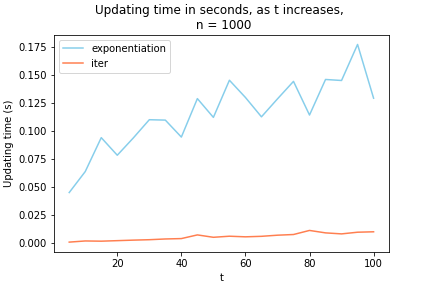
\includegraphics[width=.45\textwidth]{ThesisKI/Images/UpdatingTimeDense.png} }}%
    \qquad
    \subfloat[\centering Sparse Matrix]{{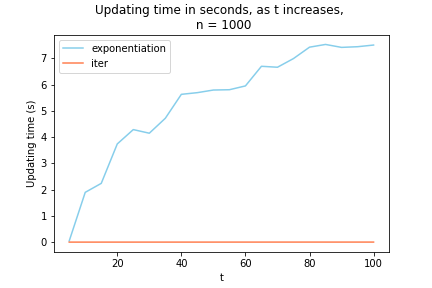
\includegraphics[width=.45\textwidth]{ThesisKI/Images/UpdatingTimeSparse.png} }}%
    \caption{Updating time}%
    \label{update:time}%
\end{figure}

Therefore the iterative method was implemented, in order to significantly speed the updating process. Furthermore, this also allows for saving all intermediate belief vectors, providing insight in the rate of convergence of the network.

However, as shown by \cite{degroot1974concensus}, the convergent belief can also be computed directly, using the eigenvector of the interaction matrix, $\T$, corresponding to $\lambda=1$. Therefore another function was made for those cases where only the convergent belief is of interest. This function gives only the convergent opinion of the network.

\subsection{$\varepsilon$-DeGroot}
\subsubsection{Standard}

The second updating rule that can be sued to converge a network is the $\varepsilon$-DeGroot variation mentioned in section [REF]\todo{ref naar section $\varepsilon$}. The general framework is the same as for standard DeGroot method: repeatedly apply the updating rule until the beliefs stop changing. However, to converge a network using this method a slight modification is necessary. First of all under the $\varepsilon$-DeGroot dynamics the belief vectors do not adhere to the standard notion of convergence as under regular DeGroot dynamics, rather, using this updating rule results in what \cite{amir2021robust} describe as \textit{alternating convergence}. That is to say, rather than one single convergent belief vector, there are two convergent belief vectors, between which the agents alternate.
Therefore, using the same condition for convergence as regular DeGroot mechanics will result in an infinite loop, as the belief vectors will alternate, ensuring there will always be a difference between the beliefs at $t$ and $t-1$. To this end, the convergence condition is changed somewhat. Rather than comparing the beliefs between $t$ and $t-1$ only, the belief vectors are compared between $t$ and $t-2$, to check whether their difference is 0, or near enough. This is also done for the beliefs at $t-1$ and $t-3$ to check whether both of the alternating belief vector have converged. As long as convergence has not occurred for both belief vectors the agents the process keeps repeating.

\subsubsection{Alternative}

The alternate $\varepsilon$-DeGroot dynamics work similarly to the standard $\varepsilon$-DeGroot updating rule, as described in [REF] \todo{ref naar alt $\varepsilon$}. Similarly, it also displays \textit{alternating} convergence, rather than the more standard notion of converge. Therefore, in order to properly detect when the network has converged the same conditions for converge are used as with the standard $\varepsilon$-DeGroot mechanics.

\subsection{Private Belief}

Another updating rule implemented allowed each individual agent to account for a private, constant, belief when updating their opinion. In the chosen implementation this private belief was chosen to be the initial belief at time $t=0$. This way agents will always place some amount of weight on their initial belief. The weight placed on this initial belief is specified by the parameter $\alpha \in [0, 1]$. Converging a network using this updating rule, follows the same process as regular DeGroot mechanics, i.e. repeatedly applying the updating rule until the belief vector no longer changes between iterations. As this updating method results in the more standard notion of convergence, opposed to \textit{alternating} convergence, no further modifications to the convergence procedure were required.

\subsection{Threshold}

Another, minor, modification to the regular DeGroot updating mechanics imposes a threshold on the updating rule, ensuring that agents do not drastically change their opinion in a single updating step. Whenever an agent changes their opinion between two time-steps they can change their opinion by no more than the given threshold, effectively limiting how volatile an agents opinion is, simulating a hesitancy in rapid, drastic, changes in opinion.

\newpage

\section{Results}
\label{results}

The results in the following section are all obtained from networks randomly generated using the same parameters. More specifically, every generated network is a directed network with an increased degree, where each agent is guaranteed to have self-link. For generating the additional degree the default distribution, as seen in Section [REF], is used.

\noindent Furthermore, the results shown for the standard deviation, distance from the assumed truth and the convergence time, are averaged over ten iterations, in order to obtain more general results. For each of the iterations a new network and initial belief vector was generated, using the same parameters as mentioned above. The graph that shows the convergence of the network towards the truth of the model is simply taken to be the last of these ten iterations.

\noindent Finally, not every updating rule showed uniform convergence. That is to say, the agents did not necessarily adopt the same opinion at the time of convergence for every updating rule. Whenever it was the case that the standard deviation of the belief vector at convergence did not equal $0$, the convergent belief was taken to be the mean of the belief vector.

\subsection{Cooperative Networks}

As can be seen in Figure \ref{coop:compare}, in a cooperative network all updating rule behave quite similar. The convergent belief differs the most for smaller network sizes. However, as the network size increases this difference dissipates, and the convergent beliefs become more and more similar, both to the other updating rules \emph{and} the assumed truth of the model.

\noindent However, while the convergent beliefs are mostly similar, the standard deviation of the convergent belief vector does differ significantly between updating rules. Where the regular and thresholded DeGroot mechanics have no deviation in the convergent belief vector, meaning there is a single convergent belief held by every agent, the other updating rules end up with a non-insignificant amount of variation in the belief vector. This means that, while the agents may no longer update their opinions, their convergent opinions still differ from each other. 

\noindent Finally, the thresholded and regular DeGroot mechanics both reach convergence in the same amount of time, while the other updating rules are significantly faster to reach the point of convergence. However, the standard and thresholded DeGroot mechanics show a clear downward trend in convergence time, which is less present for the other updating rules.

\begin{center}
    \begin{figure}[!htbp]
        \centering
        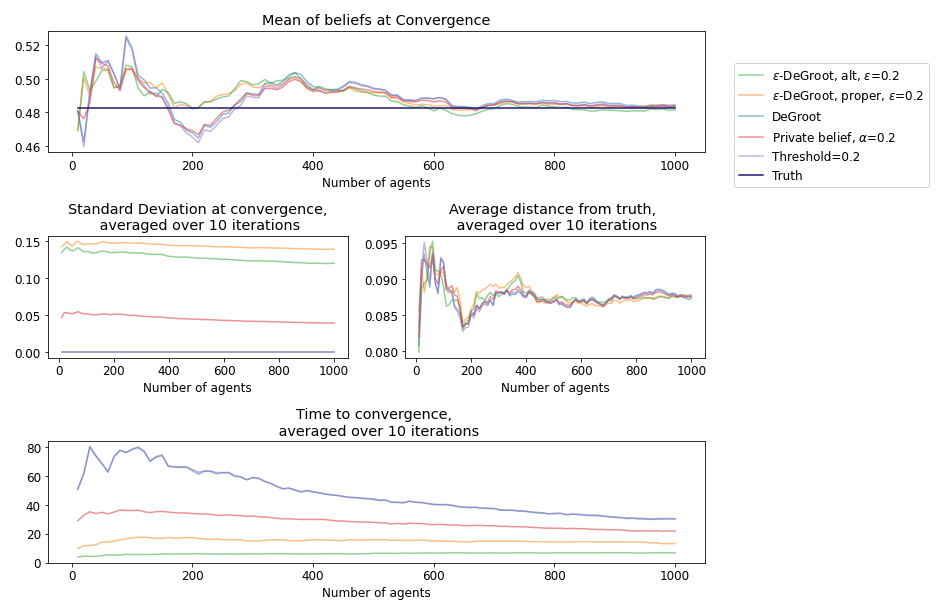
\includegraphics[width=1.2\textwidth]{ThesisKI/Images/WisdomCompare0.png}
        \caption{Convergence Behaviour Threshold Updating}
        \label{coop:compare}
    \end{figure}
\end{center}

\newpage

\subsection{Non-cooperative networks, $n=1$}

Where the different updating rules behaved in a similar fashion as the regular DeGroot updating mechanics in a fully cooperative network, significant differences start to appear when applied to a network with so much as one non-cooperative agent, as demonstrated in Figure \ref{noncoop1:compare}. 

\noindent First of all, as expected, under regular DeGroot dynamics the convergent opinion becomes that of the non-cooperative agent, and the same applies to the thresholded DeGroot mechanics. Furthermore, again as expected, this belief is uniform, held by every agent in the network, However, the other three updating mechanics exhibit vastly different behaviour. Instead of converging towards the opinion of the non-cooperative agent, the network still converges towards the truth. However, once again, this is not a uniform convergence, as there still is some deviation in the convergent belief vector, though this appears to decline ever so slightly as the network size increases. Furthermore, the standard deviation for the private belief updating rule is somewhat higher when compared to a fully cooperative network Figure \ref{coop:compare}. Also, just as in a cooperative network, the standard deviation of the private belief updating rule is significantly less than that of the $\varepsilon$-DeGroot variations.

\noindent Finally, the updating time for both the regular and the thresholded DeGroot mechanics behave nearly identical, and both display a significant increase in convergence time, whereas the other three updating rules do not appear to show significantly slower convergence. Furthermore, where it decreased as the network grew in a fully cooperative network, the convergence time only increases as the network grows in the presence of a non-cooperative agent. This increase in convergence time can be explained by the presence of the single non-cooperative agent, whose influence has to spread throughout the entire network, taking more and more time to reach every agent as the network size increases. Furthermore, this appears to be a non-factor for the other updating rules, where the non-cooperative agent is not nearly as formative, or even formative at all, for the convergent opinion, making it so that it does not significantly impact the convergence time as a result.

\begin{center}
    \begin{figure}[!htbp]
        \centering
        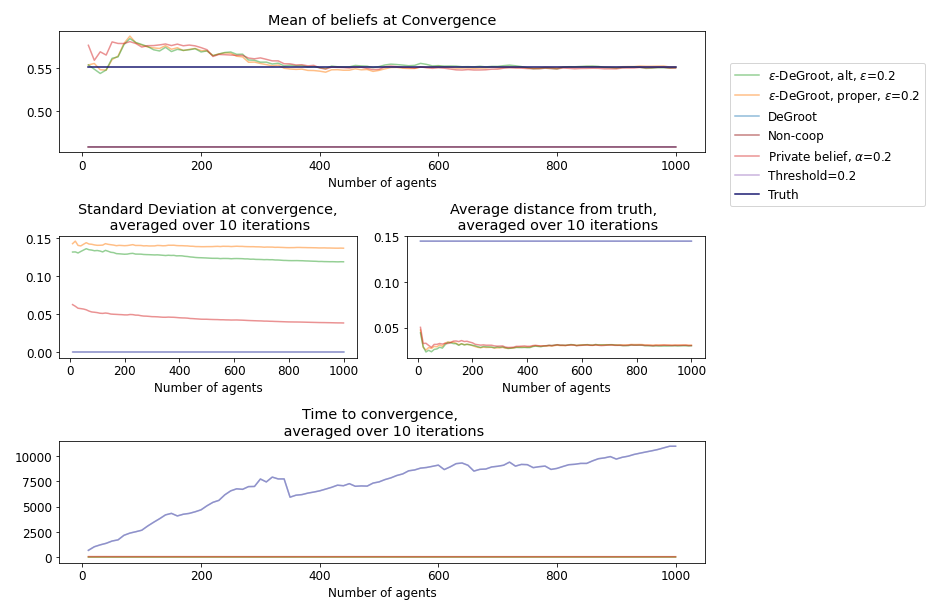
\includegraphics[width=1.2\textwidth]{ThesisKI/Images/WisdomCompare1.png}
        \caption{Convergence Behaviour Non-cooperative Network, $n=1$}
        \label{noncoop1:compare}
    \end{figure}
\end{center}

\newpage

\subsection{Non-cooperative networks, $n > 1$}

Finally, in networks with multiple non-cooperative agents there is once again a significant difference in the behaviour of the various updating rules, as seen in Figure \ref{noncoop+:compare}. Once again, both the regular and thresholded DeGroot mechanics converge towards the opinions of the non-cooperative agents, tending towards some, weighted, average between the opinions of those agents, regardless of the assumed truth. However, the effect of these non-cooperative agents is negligible to the convergent belief of the network when using the other three updating rules, all of which still converge towards the assumed truth of the network. 

\noindent However, the regular and thresholded DeGroot mechanics no longer display uniform convergence in the presence of multiple non-cooperative agents, although the standard deviation of the convergent belief vector does decrease quickly as the network size increases. On the other hand, the standard deviation of the convergent belief vector for the other updating rules does not appear to change drastically when additional non-cooperative agents are added to the network

\noindent Finally, while still significantly higher than in a fully cooperative network, the convergence time is shorter than in the presence of only one non-cooperative agent, for both the regular and thresholded DeGroot mechanics. As the number of non-cooperative in the network increases so too does their combined influence, reducing the time it takes for them to influence all cooperative agents. All the other three updating rules are still unaffected in their convergence time, as the influence of the non-cooperative agents on their updating process is very limited.

\begin{center}
    \begin{figure}[!htbp]
        \centering
        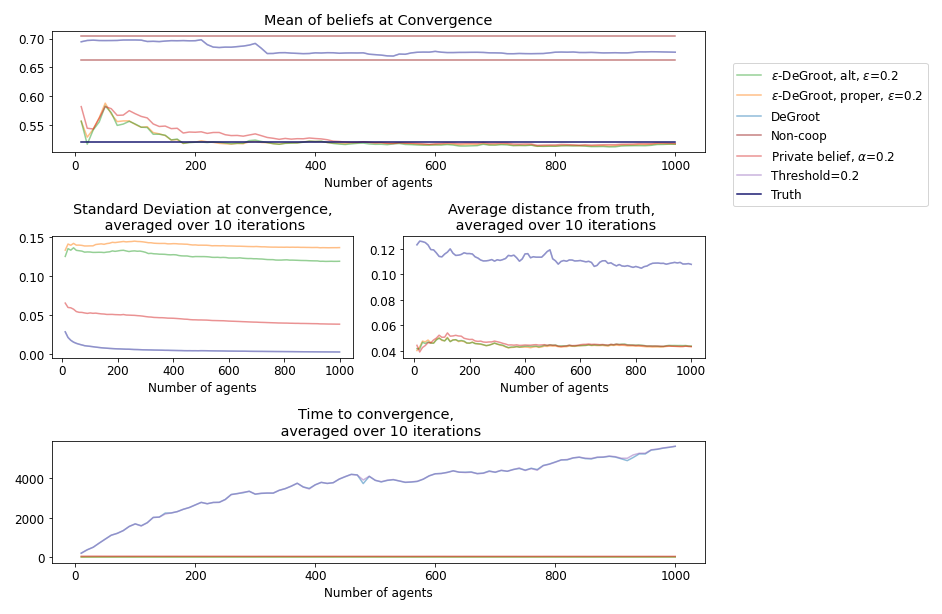
\includegraphics[width=1.2\textwidth]{ThesisKI/Images/WisdomCompare2.png}
        \caption{Convergence Behaviour Non-cooperative Network, $n>1$}
        \label{noncoop+:compare}
    \end{figure}
\end{center}

\newpage

\section{Conclusion}

The goal of the thesis was to examine the behaviour of social networks where agents update their opinions using the DeGroot mechanics, as discussed in Section [REF], and the emergent \emph{Wisdom of Crowds} effect that arises from this updating rule. More specifically, the goal was to examine the influence of any non-cooperative agents, those who refuse to change their opinion, on this effect, and how variations of the updating rule could provide a more robust updating process, more resilient to non-cooperative agents in the network. Five variations on the DeGroot mechanics, described in more detail in Section [REF], were implemented and compared in three different variations of networks; fully cooperative networks, where every agent changes their opinion; non-cooperative networks where there is only one single agent who does not change its opinion; and finally non-cooperative networks with multiple non-cooperative agents. 

\noindent As shown in Section [REF], when the network is fully cooperative the updating rules behave largely similar, all displaying the \emph{Wisdom of Crowds} effect as the network size increases. However, where the regular and thresholded DeGroot mechanics achieve a uniform converge, where every agent holds the same belief at the time of converge, both variations of the $\varepsilon$-DeGroot mechanics and the private belief updating rules do not. Instead of a single convergent belief held by every agent each agent's convergent belief is somewhat different from its neighbours'. However, their average belief still approaches the assumed truth as the network size increases, still achieving the \emph{Wisdom of Crowds} effect, though a somewhat less powerful notion than the regular DeGroot mechanics. Furthermore, the standard deviation of the private belief updating rule is significantly less than that of the $\varepsilon$-DeGroot variations.

\noindent However, strong differences occur when even a single non-cooperative agent is added to the network. Where the regular and thresholded DeGroot mechanics clearly displayed the \emph{Wisdom of Crowds} effect in a cooperative network, this effect is now completely lost. Instead, each individual agent now assumes the opinion of the single non-cooperative agent, at the time of convergence. However, this is where the other updating rules separate themselves. While they still do not achieve uniform convergence, though the variation in final opinions decreases somewhat as the network grows, the average of their belief vector at the time of convergence does not tend towards the belief of the non-cooperative agent. Rather, the \emph{Wisdom of Crowds} effect is still present, though somewhat weakened, as the average of the convergent belief vector comes ever closer to the assumed truth.

\noindent Finally, in the presence of multiple non-cooperative agents, similar results are achieved. Once again, the regular and thresholded DeGroot mechanics tend towards the opinions of the non-cooperative agents, whereas the other updating rules still exhibit the \emph{Wisdom of Crowds} effect. However, instead of one constant belief for the regular and thresholded DeGroot mechanics, the convergent belief seems to vary between different network sizes, towards some weighted average of the opinion of the non-cooperative agents in the network. Furthermore, in the presence of multiple non-cooperative agents, both the regular thresholded DeGroot mechanics no longer attain uniform convergence, though the standard deviation does tend towards $0$ as the network grows. The other three updating rules however, behave similarly in the presence of multiple non-cooperative agents as they did in networks with only one, still displaying the \emph{Wisdom of Crowds} effect, while the opinions of individual agents do still vary.

\noindent All in all, the $\varepsilon$-DeGroot variations and private belief updating mechanics are successful in making social networks more resilient to the presence of non-cooperative agents, where the thresholded DeGroot rule falls short and agents still end up adopting the opinions of the non-cooperative agents. However, these methods are not infallible, as they lose a powerful effect exhibited by the standard DeGroot mechanics. Namely, while these updating rules still converge, it is no longer the case that every agent ends up holding the same opinion, but rather, each agent adopts a somewhat different opinion from the others.

\section{Future Work}

While interesting results have come forward in this thesis there is still room for further work, as it would be desirable to find a variation on the updating rule still providing increased resilience towards non-cooperative agents, while also allowing for (more) uniform convergence.

\noindent One other variation of the DeGroot mechanics would allow the weights of the network to vary over time, which has been discussed in \cite{chatterjee1977stochastic}. One of the criticisms of the DeGroot model are its rigid weights, which do not change over time. Therefore a variation of the model where the agents can change the weight they place on others' opinions could be a more accurate reflection of the way people change their opinions, and may provide more resilience in the face of non-cooperative agents.

\noindent Furthermore, another way to combat the presence of non-cooperative agents would be to use \textquote{counter non-cooperative agents}. That is to say, non-cooperative agents specifically designed to oppose the already present non-cooperative agents in the network. The information spread by these two kinds of non-cooperative agents could possibly counteract each other, allowing the regular cooperative agents to converge towards a common opinion, and eventually the assumed truth, as the network grows sufficiently large.

\noindent Besides examining different updating rules there is also the option to look at different ways that misinformation is spread throughout a network. Another vulnerability of the \emph{Wisdom of Crowds} effect, besides the non-cooperative agents, is what \cite{amir2021robust} describe as \emph{distorted monitoring}, where every agents' initial signal is shifted over by some amount $\delta$ from the assumed truth, which can simply be implemented by using a non-zero-mean noise signal when generating the initial beliefs.

\noindent Finally, another possible direction for future work is to examine different variations of the non-cooperative agents. Where they are now represented as agents in the network receiving information from no agents but themselves, several alternatives could also be examined. First of all, a possible variation would be to represent the non-cooperative agents as a periodic influence, rather than a permanent addition to the network. Rather than permanently spreading their own opinion to their neighbours they would only spread this information every set amount of time, either to specific agents or to the network at large. 

\noindent Another natural extension of the non-cooperative agents would be to look at groups of non-cooperative agents, where the agents in this group would only receive information from other in this group while still sending information to other agents outside the group.

\newpage

\printbibliography

\newpage

\section{Appendix}
\subsection{Proof of (strong) connectedness}
\label{proof:conn}
\textbf{Base Case:} \newline
Let $S_1$ be a random social network of 1 agent, generated using the method described in \ref{generation:random}.
S is guaranteed to be fully connected, as the first agent in a network always receives a self-link.\newline

\textbf{Induction Hypothesis:}\newline
Let $S_n$ be an arbitrary, strongly connected, randomly generated network, obtained by the method described in \ref{generation:random}. Now let $S_{n+1}$ be the network that is obtained by growing the network $S_n$ by one agent. We now want to prove that if $S_{n+1}$ is grown from $S_n$ using the method from \ref{generation:random}, $S_{n+1}$ is also strongly connected.\newline

To grow the network $S_n$ by one agent, the agent $n+1$ is added to the network, with two guaranteed links, one incoming and one outgoing. Let the $i$ and $j$ be the arbitrary agents involved in these links, respectively. By the generation procedure outlined in \ref{generation:random}, these agents are guaranteed to be present in $S_n$. However, by our induction hypothesis we now that $S_n$ is strongly connected, therefore there exists a directed path from $i$ and $j$ to any other agent in the network. Therefore, as agent $n+1$ has an incoming link from agent $i$, there exists an incoming path from any agent in the network to $n+1$, and, furthermore, as $n+1$ has an outgoing link to agent $j$, there also exists an outgoing path to any agent in the network. Therefore, as there exists a directed path to any agent in the network from agent $n+1$, $S_{n+1}$ must be strongly connected.\newline
Therefore, as $S_n$ and $S_{n+1}$ were arbitrary networks, it must be the case that any network generated using this method must be strongly connected.\newline


%\bibliographystyle{apa}
%\bibliography{references.bib}
\end{document}



